\documentclass[article]{beamer}
\usetheme{Warsaw}
\setbeamertemplate{footline}[frame number]

\usefonttheme[]{serif}
\usepackage{amsmath, latexsym, color, graphicx, amssymb, bm, here}
\usepackage{epsf, epsfig, pifont,tikz,subfigure}
\usepackage{graphics, calrsfs}
\usepackage{times}
\usepackage{fancybox,calc}
\usepackage{palatino,mathpazo}
\usepackage{amsfonts}
\usepackage{sidecap}
\usepackage{listings}
\usepackage{hyperref}
\usepackage{algorithm, algorithmic}

\title{Graph Theory: DFS Applications}
\author{David Jacobo \\ \href{mailto:jguillen@cimat.mx}{jguillen@cimat.mx}}
\date{\scriptsize{\today}}

\AtBeginSection[]
{
  \begin{frame}{Outline}
    \tableofcontents[currentsection]
  \end{frame}
}

\begin{document}

%%%%%%%%%%%%%%%%%%%%%%%%%%%%%%
\maketitle			
			
%%%%%%%%%%%%%%%%%%%%%%%%%%%%%%
\begin{frame}
\frametitle{Definition}
\begin{center}
\huge
	G = (V, E)
	
\vspace{8mm}	
	
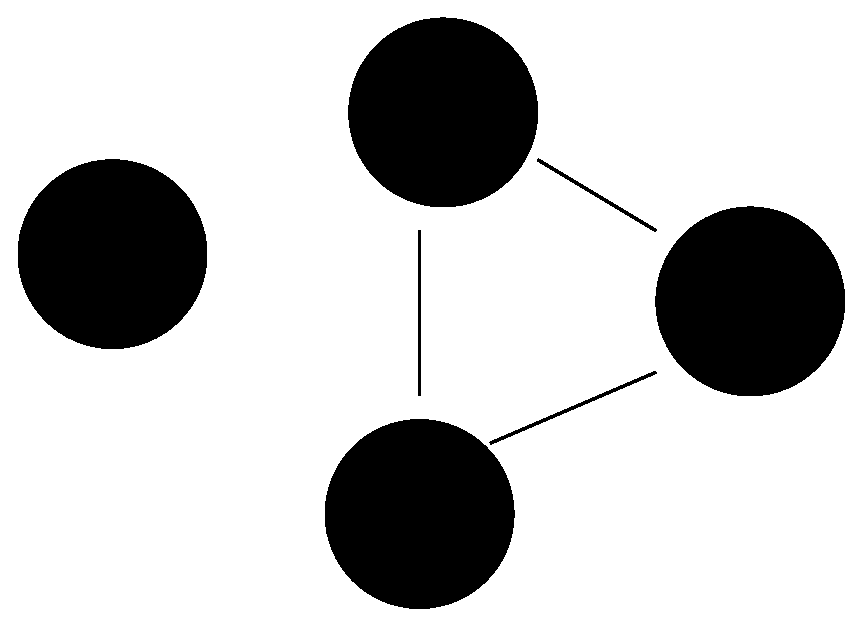
\includegraphics[scale=0.3]{./figures/graph.eps}
\end{center}
\end{frame}

%%%%%%%%%%%%%%%%%%%%%%%%%%%%%%

\section{Flood fill}
\subsection{Intuition}
\begin{frame}
	\frametitle{Flood fill}
	Using DFS and starting from a vertex \textbf{u}, find all the reachable vertices either directly or indirectly.
	
	\vspace{5mm}
	
	%insert image here
	\begin{columns}
	\column{.5\textwidth}
	Usage:
	\begin{itemize}
		\item Component labeling
		\item Reachability test
	\end{itemize}
	\column{.5\textwidth}
	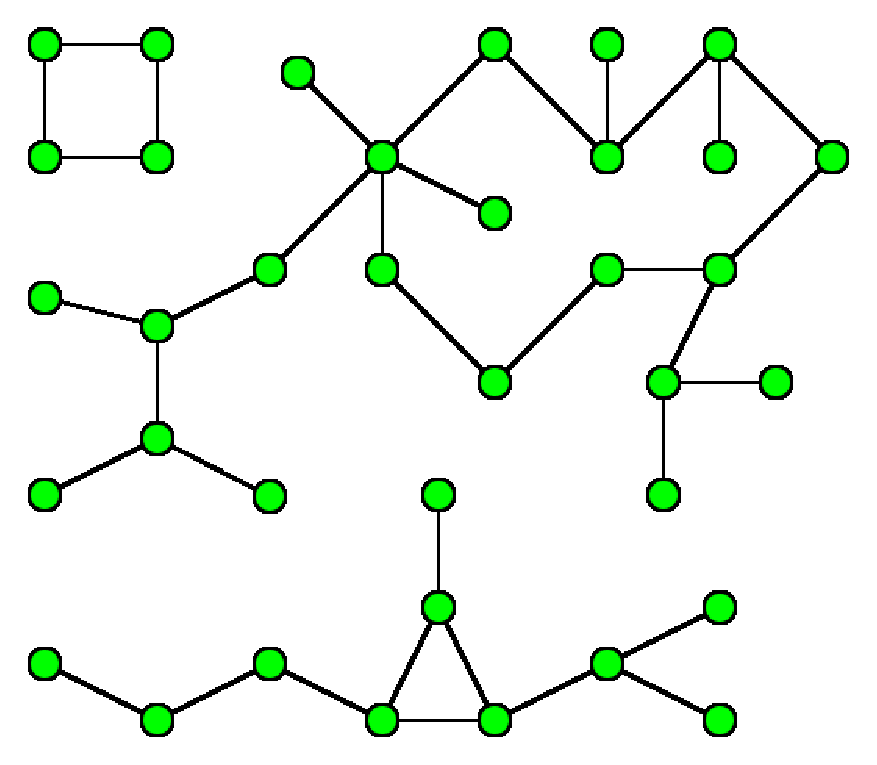
\includegraphics[scale=0.3]{./figures/forest.eps}
	\end{columns}
\end{frame}

%%%%%%%%%%%%%%%%%%%%%%%%%%%%%%%
\subsection{Algorithm}
\begin{frame}
	\frametitle{Algorithm}
	
		\begin{algorithm}[H]
		\begin{algorithmic}[1]
		\STATE $\forall$ $u$ $\in$ $V$, $u_{traversed}$ $\gets$ false		
		\STATE $component \gets$ 0		
		\FOR{$u \in V$}
		\IF{$u_{traversed}$ = false}
		\STATE dfs $(u, component)$
		\STATE $component \gets component + 1$
		\ENDIF
		\ENDFOR		
		
		\end{algorithmic}
		\caption{Flood fill}
		\label{alg:seq}
		\end{algorithm}	
	
\end{frame}


\begin{frame}
	\frametitle{Algorithm}
	
		\begin{algorithm}[H]
		\begin{algorithmic}[1]
		\STATE $u_{traversed} \gets$ true
		\STATE $u_{component} \gets component$			
		\FOR{$v$ $\in$ $u_{neighbours}$ }
		\IF{$v_{traversed}$ = false}
		\STATE dfs$(v, component)$
		\ENDIF
		\ENDFOR
		
		\end{algorithmic}
		\caption{dfs$(u, component)$}
		\label{alg:seq}
		\end{algorithm}	
	
\end{frame}
%%%%%%%%%%%%%%%%%%%%%%%%%%%%%%%%%

\section{Bi-coloring}
\subsection{Intuition}
\begin{frame}
	\frametitle{Bi-coloring}
	Can a graph be labeled with 2 'colors'?
	
	\vspace{5mm}
	%insert image here
	
	\begin{columns}
	\column{.6\textwidth}
	Usage:
	\begin{itemize}
		\item Bipartite matching is based on this algorithm as pre-processing in the case the 2 groups are not given in beforehand.
	\end{itemize}
	\column{.4\textwidth}
	\includegraphics[scale=0.2]{./figures/bipartite.eps}
	\end{columns}
\end{frame}

%%%%%%%%%%%%%%%%%%%%%%%%%%%%%%%%%

\subsection{Algorithm}
\begin{frame}
	\frametitle{Algorithm}
	\begin{algorithm}[H]
		\begin{algorithmic}[1]
		\STATE $\forall$ $u$ $\in$ $V$, $u_{color}$ $\gets$ -1				
		\FOR{$u$ $\in$ $V$}
		\IF{$u_{color}$ = -1}
		\STATE $u_{color}$ $\gets$ 1
		\STATE dfs-color $(u)$
		\ENDIF
		\ENDFOR		
		
		\end{algorithmic}
		\caption{Bi-coloring}
		\label{alg:seq}
		\end{algorithm}
\end{frame}

\begin{frame}
	\frametitle{Algorithm}
	\begin{algorithm}[H]
		\begin{algorithmic}[1]
		\FOR{$v$ $\in$ $u_{neighbours}$ }
		\IF{$v_{color}$ = -1}
		\STATE $v_{color} \gets 1 - u_{color}$
		\STATE dfs-color$(v)$
		\ELSIF{$v_{color} = u_{color}$}
		\STATE Fail, not bipartite!
		\ENDIF
		\ENDFOR
		\end{algorithmic}
		\caption{dfs-color$(u)$}
		\label{alg:seq}
		\end{algorithm}
\end{frame}

%%%%%%%%%%%%%%%%%%%%%%%%%%%%%%

\section{Cycle detection}
\subsection{Intuition}
\begin{frame}
	\frametitle{Cycle detection}
	A cycle could be described as: \textbf{$v_{0}, v_{1}, v_{2} ... v_{n}, v_{0}$}. Could you detect a cycle on the graph, if present?
	
	\vspace{5mm}
	
	\begin{columns}
	\column{.5\textwidth}
	Usage:
	\begin{itemize}
		\item Topological sorting
		\item Tree detection
		\item Strong connected components (on a directed graph)
		\item Bridges detection 
		\item Articulation point detection
	\end{itemize}
	\column{.5\textwidth}
	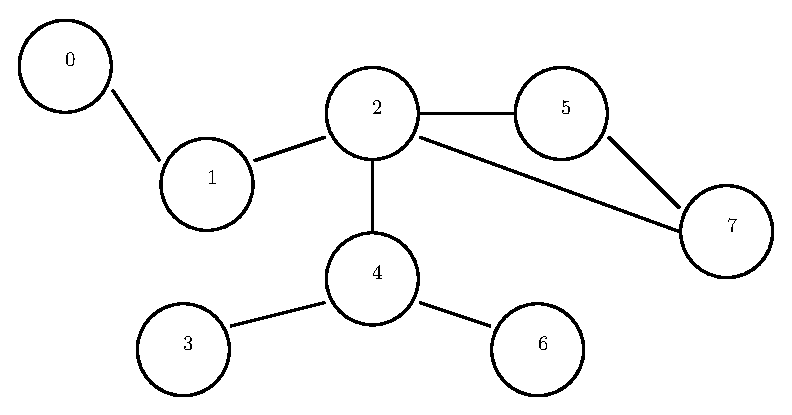
\includegraphics[scale=0.4]{./figures/path_cycle.eps}
	\end{columns}
\end{frame}

%%%%%%%%%%%%%%%%%%%%%%%%%%%%%%

\subsection{Algorithm}
\begin{frame}
	\frametitle{Algorithm}
	\begin{algorithm}[H]
		\begin{algorithmic}[1]
		\STATE $\forall$ $u$ $\in$ $V$, $u_{color}$ $\gets$ BLACK, $u_{parent} \gets -1$				
		\FOR{$u$ $\in$ $V$}
		\IF{$u_{color}$ = BLACK}
		\STATE dfs-cycle $(u)$
		\ENDIF
		\ENDFOR		
		
		\end{algorithmic}
		\caption{Cycle detection}
		\label{alg:seq}
		\end{algorithm}
\end{frame}

\begin{frame}
	\frametitle{Algorithm}
	\begin{algorithm}[H]
		\begin{algorithmic}[1]
		\STATE $u_{color} \gets$ GRAY
		\FOR{$v$ $\in$ $u_{neighbours}$ }
		\IF{$v_{color}$ = BLACK}
		\STATE $v_{parent} \gets u$
		\STATE dfs-cycle$(v)$
		\ELSIF{$v_{color}$ = GRAY AND $u_{parent} \neq v$}
		\STATE We found a cycle!
		\ELSIF{$v_{color}$ = WHITE}
		\STATE We don't care about this case for cycles
		\ENDIF
		\ENDFOR
		\STATE $u_{color} \gets$ WHITE
		\end{algorithmic}
		\caption{dfs-cycle$(u)$}
		\label{alg:seq}
		\end{algorithm}
\end{frame}

%%%%%%%%%%%%%%%%%%%%%%%%%%%%%%
\begin{frame}[plain]
\frametitle{}
\begin{center}
\Huge{\color{blue}{Q \& A}} \\
\vspace{5mm}
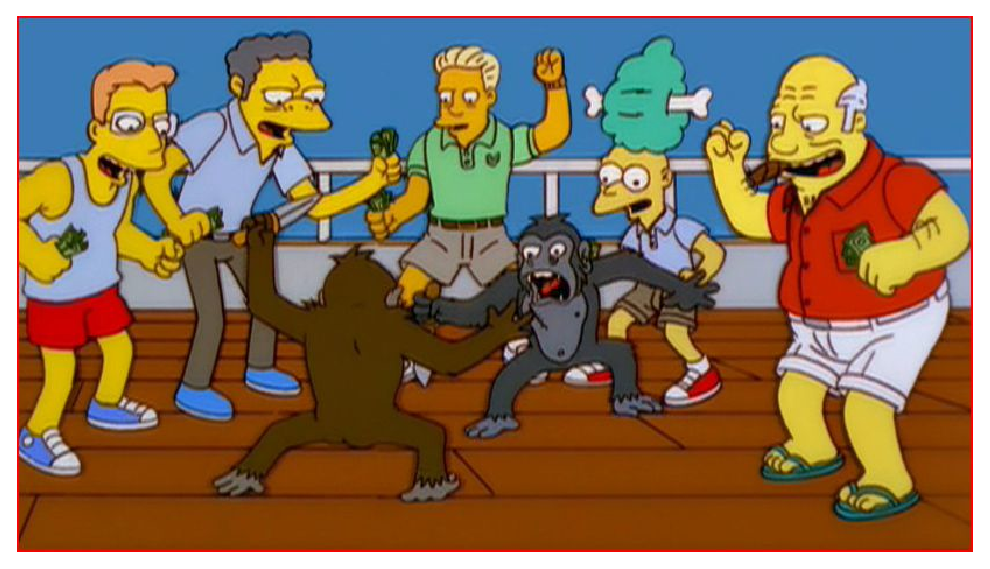
\includegraphics[scale=0.4]{./figures/monkey_fight.eps}
\end{center}
\end{frame}

%%%%%%%%%%%%%%%%%%%%%%%%%%%%%%%%
\begin{frame}[plain]
	\textbf{References}
	\begin{itemize}
		\item \href{https://sites.google.com/site/stevenhalim/}{Competitive Programming site}
		\item \href{https://github.com/davidjacobo/algorists/}{Algorists' repository}
	\end{itemize}
\end{frame}
\end{document}
